\documentclass[10pt,twocolumn,letterpaper]{article}

\usepackage[margin=0.75in]{geometry}
\usepackage{times}
\usepackage{graphicx}
\usepackage{amsmath,amssymb}
\usepackage{booktabs}
\usepackage{microtype}
\usepackage{enumitem}
\usepackage[hidelinks]{hyperref}

\setlength{\columnsep}{0.25in}
\setlist[itemize]{leftmargin=*, topsep=2pt, itemsep=1pt, parsep=0pt}
\setlength{\textfloatsep}{8pt plus 2pt minus 2pt}
\setlength{\floatsep}{8pt plus 2pt minus 2pt}
\setlength{\abovecaptionskip}{4pt}
\setlength{\belowcaptionskip}{-2pt}

\title{SmartReach-HSM: Train-Free Same-Source Multimodal Grounding for Single-RGB Assistive Grasp Dialogue}
\author{Anonymous COMP5523 Project Team}
\date{}

\begin{document}
\maketitle

\begin{abstract}
Assistive grasp guidance from a single RGB camera is difficult because the system must resolve three relations at once: which object is relevant, where the user's hand lies relative to it, and whether the hand must move forward or backward to reach it. We address this constraint by decomposing each RGB frame into same-source detection, hand-pose, and monocular-depth cues, while retaining the original RGB image as the appearance reference. The key design choice is \emph{train-free multimodal grounding}: all backbones remain frozen, and task adaptation is pushed into an inference-time interface that assigns distinct roles to the RGB image, depth image, detection JSON, hand-pose JSON, and short dialogue history. Following the context-space view of training-free adaptation in Training-Free GRPO~\cite{cai2025tfgrpo}, we treat train-free not as prompt hacking or as rollout-based optimization, but as a deliberate relocation of task adaptation from parameter updates to structured inference-time priors. The implemented prototype transcribes user speech, captures a fresh frame, derives same-source cues, queries GLM-4.6V with two images plus structured text evidence, and speaks the returned Chinese guidance directly. This yields an inspectable single-camera speech-to-speech system that avoids cross-sensor calibration and task-specific fine-tuning while remaining grounded in actionable spatial evidence.
\end{abstract}

\section{Introduction}
For a visually impaired user, a useful grasping assistant must do more than name objects. It must identify the relevant object, relate that object to the user's hand, resolve front-back ambiguity, and express the result as a short spoken instruction that can be executed immediately. A generic RGB scene captioner fails on this requirement because it may describe the table correctly while still failing to answer the operational question: \emph{where is the target relative to my hand, and how should I move next?}

Many embodied-assistance systems reduce this ambiguity by adding sensors, calibration, or task-specific training. Those choices are effective, but they also increase hardware cost, deployment complexity, and data dependence. We study the opposite corner of the design space: a fixed single RGB camera, frozen perception and language backbones, and inference-time composition only. The challenge is then not merely to run a multimodal model, but to construct an evidence interface rich enough for grounded grasp dialogue under this severe sensing budget.

Our answer is \emph{same-source multimodal grounding}. From one RGB frame we derive three aligned auxiliary cues: open-vocabulary object detections, 2D hand landmarks, and dense monocular depth. Inspired by homologous multimodal learning, where multiple modalities are derived from the same source and exploited because they preserve complementary views of one scene~\cite{xie2023hmjnd}, we use same-source cues not to build a learned fusion network, but to preserve alignment between semantics, embodiment, and geometry without cross-sensor registration.

The second design principle is that this bridge from perception to language must be \emph{train-free}. Training-Free GRPO argues that behavior adaptation can be shifted from parameter space to context space by injecting priors at inference time rather than updating model weights~\cite{cai2025tfgrpo}. We adopt that non-parametric viewpoint, but not the algorithmic machinery of Training-Free GRPO itself: our system does not perform grouped rollouts, semantic-advantage extraction, or experience-library updates. Instead, it instantiates a fixed assistive prior that tells the multimodal model how to interpret each cue and how to answer.

The deployed loop is therefore simple and conversational: ASR produces the latest user utterance, the current RGB frame is captured, same-source cues are extracted, a structured multimodal prompt is assembled, GLM-4.6V returns Chinese guidance, and TTS speaks the response. Within that loop, the central contribution is not a new trained policy, but a coherent interface that converts one RGB frame into grounded assistive dialogue.

Our contributions are threefold: (i) a same-source cue decomposition that recovers semantic, embodied, and geometric evidence from one RGB view; (ii) a train-free inference interface that shifts task adaptation from parameter updates to structured context injection; and (iii) an inspectable single-camera prototype for assistive grasp dialogue with direct speech output.

\section{Positioning Relative to Prior Work}
\textbf{Same-source multimodality.} Prior homologous multimodal work shows that multiple useful cues can be derived from one source and exploited jointly because they remain naturally aligned~\cite{xie2023hmjnd}. That literature usually learns explicit fusion and alignment modules over those cues. Our setting is different: we adopt the same-source principle as a systems design choice for assistive grounding, but we deliberately avoid learned multimodal fusion. The practical question here is not how to train a better feature backbone, but how to organize frozen same-source evidence so that a deployed multimodal model can produce grounded instructions.

\textbf{Train-free adaptation.} Training-Free GRPO frames training-free adaptation as moving policy improvement from parameter space to context space~\cite{cai2025tfgrpo}. In that work, the context prior is \emph{learned} through grouped rollouts and an evolving experience library. Our system uses the same high-level principle---non-parametric behavior shaping at inference time---but with a fixed task prior rather than an optimized token prior. This distinction matters: the novelty of our system is not rollout-based optimization, but a train-free assistive interface over frozen specialist modules.

\begin{figure*}[t]
    \centering
    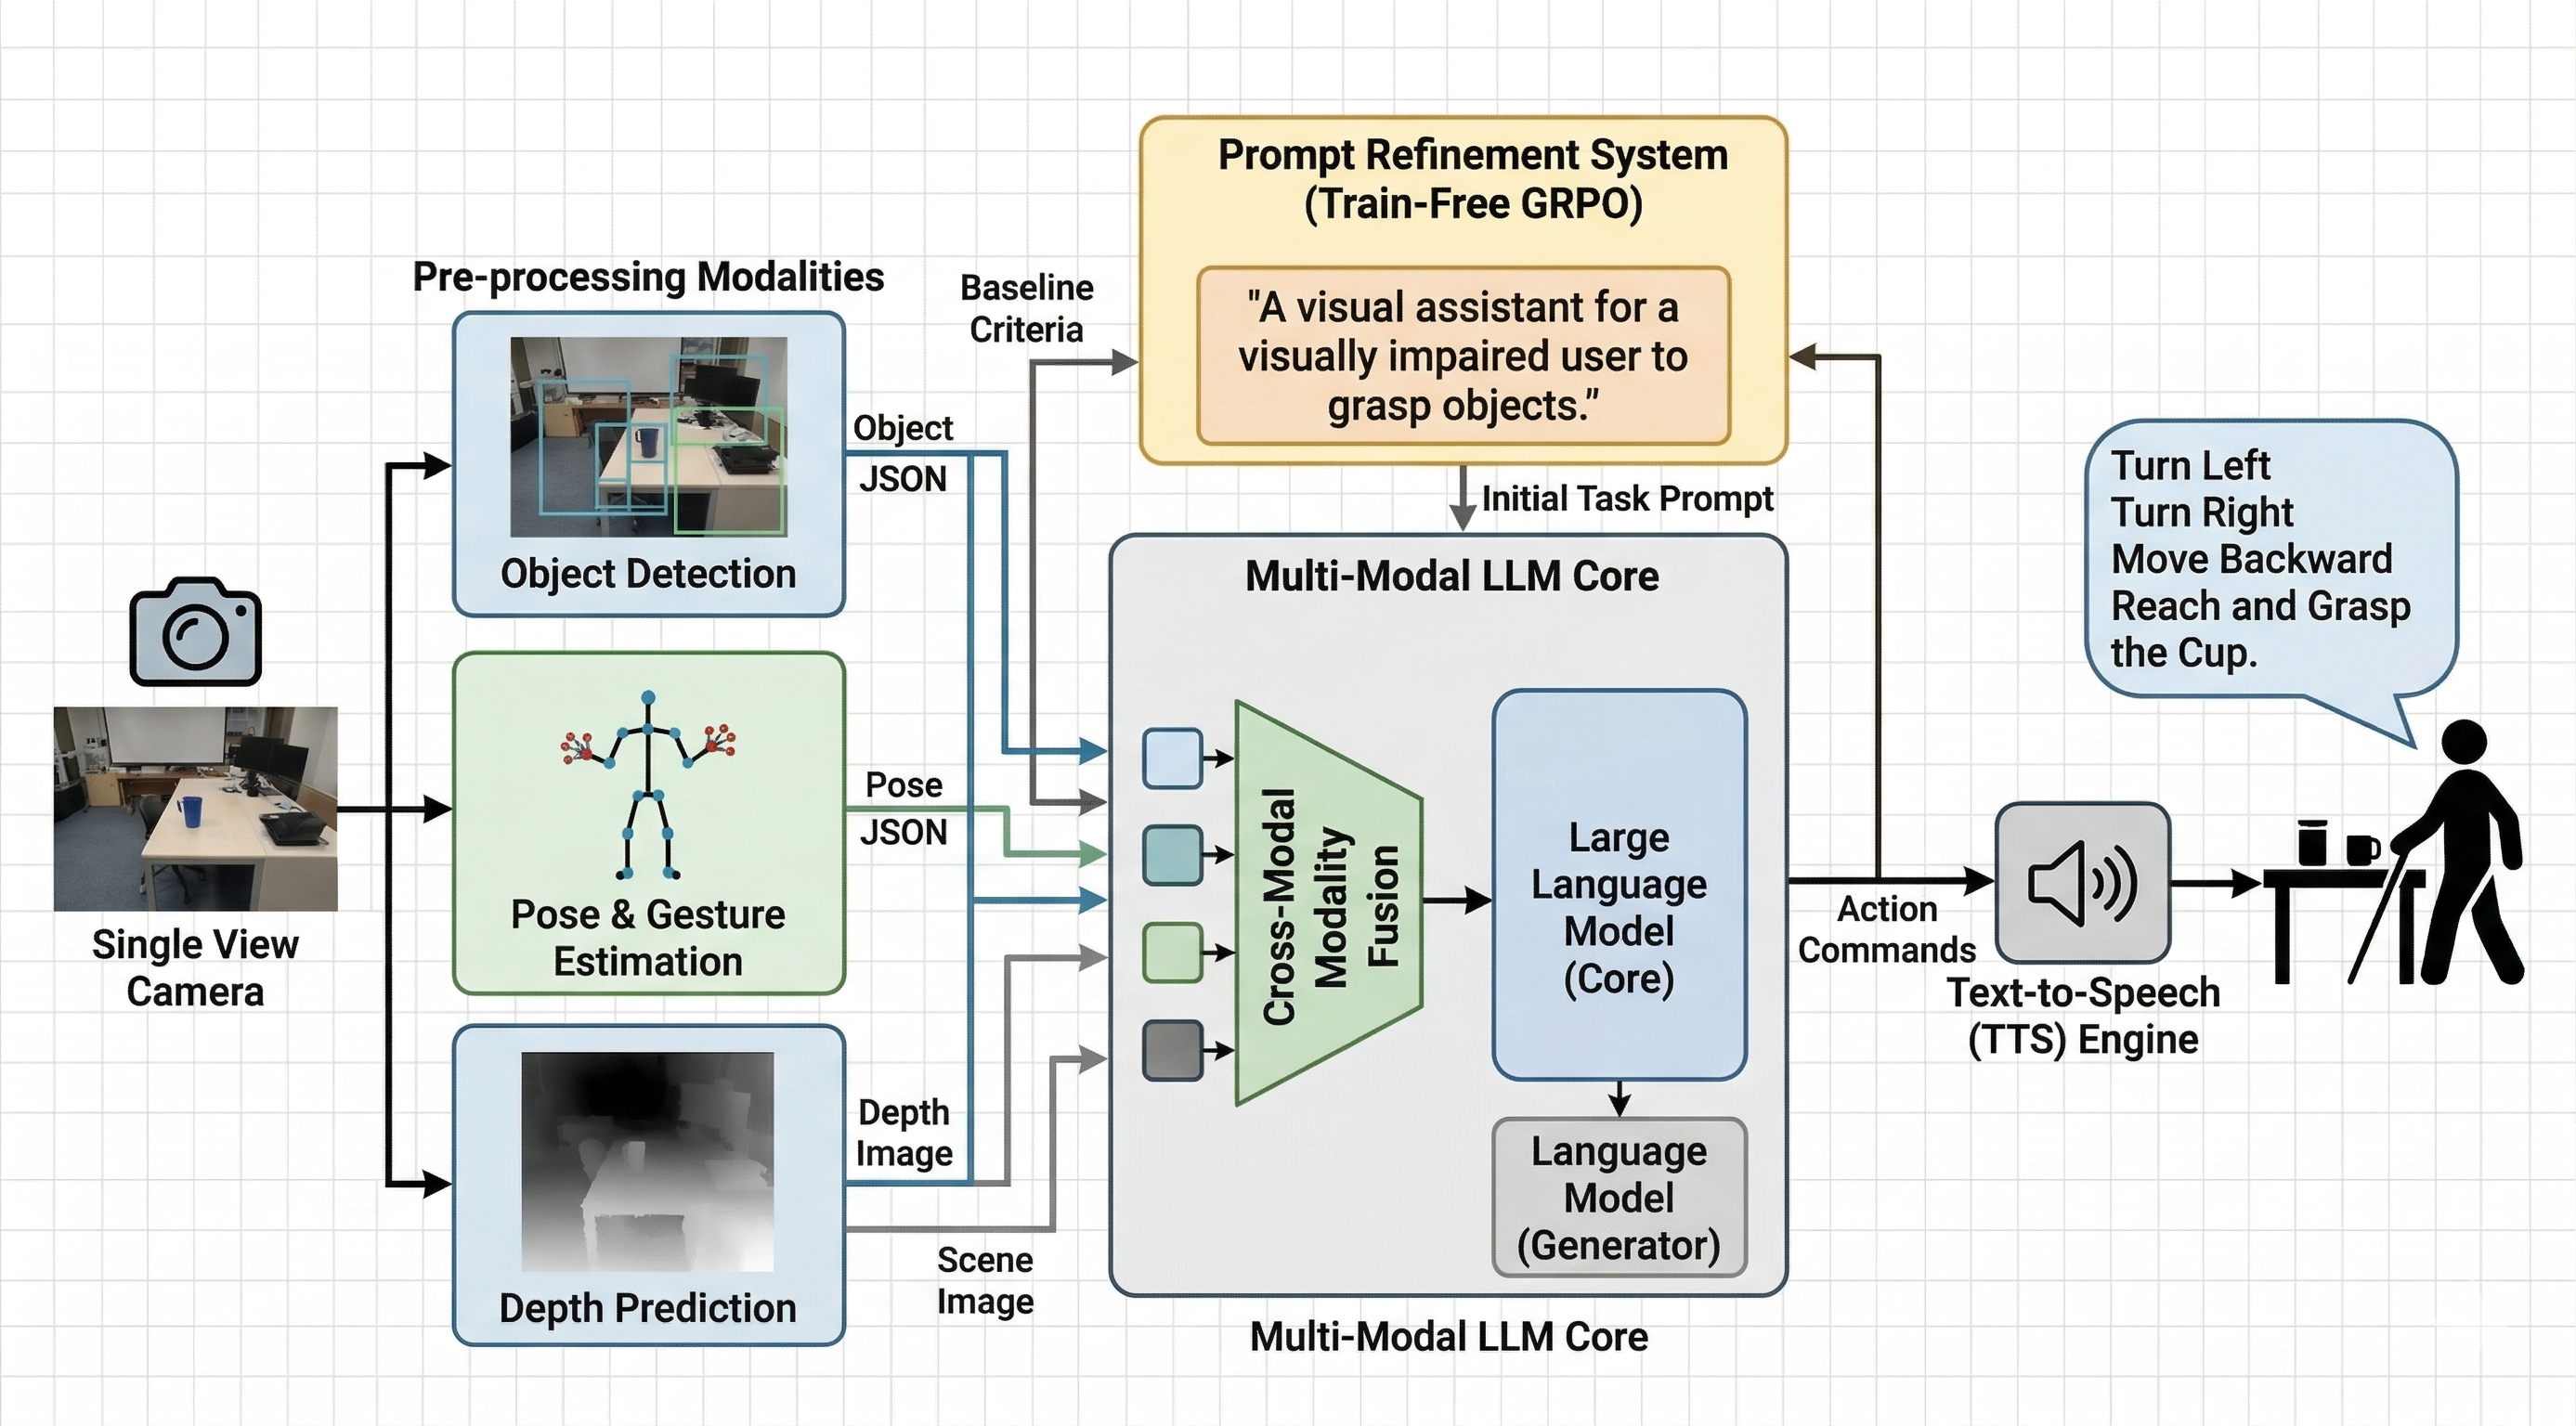
\includegraphics[width=0.97\textwidth]{pipeline.png}
    \caption{Pipeline of SmartReach-HSM. A single RGB view is decomposed into the original RGB image, object-detection evidence, hand-pose evidence, and monocular depth. These same-source cues are then organized by a train-free inference interface before entering the multimodal reasoning stage. In the deployed system, the online loop is ASR $\rightarrow$ current-frame capture $\rightarrow$ same-source cue extraction $\rightarrow$ structured multimodal prompting $\rightarrow$ GLM-4.6V response $\rightarrow$ Chinese TTS.}
    \label{fig:pipeline}
\end{figure*}

\section{Method}
\subsection{Problem Setting}
At dialogue turn $t$, the user speaks a query $q_t$ and the system captures the current RGB frame $I_t$. From that same frame, it derives an object-detection representation $D_t^{obj}$, a hand-pose representation $D_t^{hand}$, and a monocular depth image $I_t^{depth}$. Let $H_t$ denote the short dialogue history retained from previous user and assistant turns. The deployed system produces a directly speakable response
\begin{equation}
y_t = \mathcal{M}(q_t, H_t, I_t, I_t^{depth}, D_t^{obj}, D_t^{hand}),
\end{equation}
where $y_t$ should be concise, spatially grounded, and useful for continuing a grasp-oriented interaction.

This formulation emphasizes an important scope choice. The task is not generic scene description; it is executable spoken guidance conditioned on object identity, hand location, and relative geometry under a single-view constraint.

\subsection{Same-Source Cue Decomposition}
The first stage of the system converts one RGB observation into task-minimal evidence streams:
\begin{equation}
\begin{aligned}
D_t^{obj} &= f_{det}(I_t), \\
D_t^{hand} &= f_{hand}(I_t), \\
I_t^{depth} &= f_{depth}(I_t).
\end{aligned}
\end{equation}

\textbf{Detection cue.} We use Grounding DINO~\cite{liu2023groundingdino} to transform the RGB frame into open-vocabulary detections represented as category labels, confidence scores, and 2D bounding boxes. This cue resolves the semantic-anchor problem: which object is relevant, and where is it in the image plane.

\textbf{Hand-pose cue.} We use MediaPipe hand tracking~\cite{lugaresi2019mediapipe} to estimate handedness and up to 21 2D landmarks from the same RGB frame. This cue resolves the embodiment problem: where the user's acting effector is, so that guidance can be issued relative to the hand rather than relative to the camera alone.

\textbf{Depth cue.} We use Depth Anything V2~\cite{yang2024depthanythingv2} to predict a dense monocular depth map from the same RGB frame and resize it back to the original image resolution. This cue resolves the front-back ambiguity that 2D appearance and boxes cannot settle by themselves. In our implementation, the depth map is primarily used as relative geometry, not as calibrated metric distance.

These modalities are chosen because each addresses a distinct failure mode of RGB-only guidance. Detection answers \emph{what} and \emph{where} in image coordinates; hand pose answers \emph{where the user acts}; depth answers \emph{whether the hand is in front of or behind the target}. Their complementarity is therefore task-driven, not decorative.

\subsection{Aligned Spatial Evidence}
The deeper benefit of same-source decomposition is not merely that it removes calibration. Because all cues are derived from the same frame, they share one image-plane reference and can be reduced to compact spatial evidence. In the implementation, the detection box center defines a target anchor, a palm-center estimate is computed from the hand landmarks, and the depth map is sampled near both anchors. This yields interpretable relation variables such as horizontal offset, vertical offset, and relative depth difference between the target and the hand.

These compact variables are not introduced as a separate trained representation. They arise deterministically from aligned same-source cues and explain why the modality set is sufficient for grasp dialogue. Even when the deployed dialogue path sends only RGB, depth, and structured JSON to GLM-4.6V, the underlying same-source alignment still provides a physically meaningful coordinate interface for debugging, overlay rendering, and prompt-side spatial interpretation.

This distinction is important for paper logic. We do \emph{not} claim a new learned multimodal fusion architecture. Rather, the system uses same-source alignment to make semantic, embodied, and geometric evidence mutually interpretable before language generation.

\subsection{Train-Free Inference Interface}
The second stage is the train-free interface that binds these cues to multimodal reasoning. Here, \emph{train-free} has a strict meaning: no task-specific gradient updates are performed for ASR, object detection, depth estimation, hand tracking, or the multimodal LLM. Adaptation is moved entirely into inference-time context design, in the spirit of context-space rather than parameter-space adaptation~\cite{cai2025tfgrpo}.

At the same time, our method is deliberately narrower than Training-Free GRPO. Training-Free GRPO learns an evolving token prior from grouped rollouts, semantic advantages, and an external experience library~\cite{cai2025tfgrpo}. We do not perform any of those steps. The prior in SmartReach-HSM is fixed and task-structured. It is implemented by three coordinated decisions:
\begin{itemize}
    \item \textbf{Modality-role assignment.} The prompt explicitly tells the model to use the depth image for front-back reasoning, detection JSON for object identity and 2D location, hand-pose JSON for hand position and posture cues, and RGB for scene appearance consistency.
    \item \textbf{Dialogue prior.} A short text history of previous user and assistant turns is retained so that follow-up questions such as ``What should I do next?'' or ``How about now?'' can be interpreted in context.
    \item \textbf{Assistive response prior.} The model is instructed to produce direct Chinese guidance that prioritizes relative position, next-step motion, and, when justified by hand evidence, coarse hand-shape suggestions.
\end{itemize}

The key claim is therefore precise: our system relocates task adaptation from weight updates to a structured multimodal prior over frozen modules.

\subsection{Deployed Dialogue Loop}
Figure~\ref{fig:pipeline} summarizes the pipeline. The online path follows a strict conversational loop: a user utterance is transcribed, a fresh RGB frame is captured, the three same-source cues are extracted, and GLM-4.6V receives two images plus structured text evidence. Concretely, the multimodal model sees the original RGB image, the normalized depth image, serialized detection JSON, serialized hand-pose JSON, and recent dialogue history. It then returns the response text that is spoken directly by TTS.

This deployment choice deliberately removes parser-driven user-facing control logic from the main interaction path. The multimodal model is asked to answer the user's current request using current-frame evidence, rather than being wrapped by a rule engine that rewrites speech. The result is a cleaner speech-to-speech interaction that better matches the target assistive scenario.

The figure should therefore be read as an evidence-interface diagram, not as a claim that we train a new multimodal backbone. The contribution is the structured arrangement of aligned evidence under a train-free deployment constraint.

\section{Implemented Prototype, Inspectability, and Limitations}
The current prototype is implemented in Python with Whisper large-v3-turbo for ASR~\cite{radford2023whisper}, Grounding DINO for detection~\cite{liu2023groundingdino}, Depth Anything V2 for monocular depth~\cite{yang2024depthanythingv2}, MediaPipe for hand landmarks~\cite{lugaresi2019mediapipe}, and GLM-4.6V as the multimodal reasoner. Importantly, the active GLM backend sends two images---RGB and normalized depth---together with the structured prompt, so the system does not rely on a collage-style dashboard as the primary model input.

The system is also designed to be inspectable. For each dialogue turn, the implementation logs the RGB image, the depth image, the prompt text, and the structured payload delivered to the multimodal model. This matters scientifically because a train-free method should be debuggable at the interface level: if grounding fails, the developer can inspect the exact evidence that was exposed to the model rather than treating the multimodal call as opaque.

This report is intentionally scoped as a systems-and-method paper, not a benchmark paper. We do not claim quantitative superiority, robotic grasp success rates, or user-study outcomes here. The current design also inherits the limitations of its single-view setting: monocular depth is relative rather than metric; 2D hand landmarks support only coarse posture inference; and the same-source choice couples failure modes, so blur, occlusion, or a poor viewpoint can jointly degrade detection, depth, and hand estimates. These limitations do not negate the method, but they define the honest boundary of what the present prototype demonstrates.

\section{Conclusion}
We presented SmartReach-HSM, a single-camera assistive grasp dialogue system built around two linked ideas: same-source cue decomposition and train-free multimodal grounding. From one RGB frame, the system derives aligned semantic, embodied, and geometric evidence; from those frozen cues, it constructs an inference-time interface that guides a multimodal LLM without task-specific parameter updates. The main contribution is therefore not a new learned grasp policy, but a coherent and inspectable route from single-RGB perception to grounded assistive speech.

{\small
\bibliographystyle{ieeetr}
\bibliography{references}
}

\end{document}
